\documentclass[letterpaper]{article} % DO NOT CHANGE THIS
\usepackage{aaai20}  % DO NOT CHANGE THIS
\usepackage{times}  % DO NOT CHANGE THIS
\usepackage{helvet} % DO NOT CHANGE THIS
\usepackage{courier}  % DO NOT CHANGE THIS
\usepackage[hyphens]{url}  % DO NOT CHANGE THIS
\usepackage{graphicx} % DO NOT CHANGE THIS
\urlstyle{rm} % DO NOT CHANGE THIS
\def\UrlFont{\rm}  % DO NOT CHANGE THIS
\usepackage{graphicx}  % DO NOT CHANGE THIS
\frenchspacing  % DO NOT CHANGE THIS
\setlength{\pdfpagewidth}{8.5in}  % DO NOT CHANGE THIS
\setlength{\pdfpageheight}{11in}  % DO NOT CHANGE THIS
\usepackage{subfig}

%%%%%%%%%%%%
\usepackage[utf8]{inputenc} % allow utf-8 input
\usepackage[T1]{fontenc}    % use 8-bit T1 fonts
\usepackage{booktabs}       % professional-quality tables
\usepackage{amsfonts}       % blackboard math symbols
\usepackage{nicefrac}       % compact symbols for 1\2, etc.
\usepackage{microtype}      % microtypography
\usepackage{graphicx}
%\usepackage{natbib}
\usepackage{ascmac}
\usepackage{amsmath,amssymb,amsfonts,array}
\usepackage{theorem}
\usepackage{bm}
\usepackage{mleftright}
\mleftright
\usepackage{braket}
\usepackage{extarrows}
\usepackage{booktabs}
\usepackage{algorithm,algorithmic}
\usepackage{tikz}
\usepackage{color}
\usepackage{xcolor}
\usepackage{overpic}
\usepackage{multirow}
\usepackage{xr-hyper}
\usepackage{hyperref}
\usepackage[capitalise,noabbrev]{cleveref}

%%%% for xy-hyper
\makeatletter
\newcommand*{\addFileDependency}[1]{% argument=file name and extension
  \typeout{(#1)}
  \@addtofilelist{#1}
  \IfFileExists{#1}{}{\typeout{No file #1.}}
}
\makeatother
 
\newcommand*{\myexternaldocument}[2][]{%
    \externaldocument[#1]{#2}%
    \addFileDependency{#2.tex}%
    \addFileDependency{#2.aux}%
}

%%%% for showkey of cleveref
% \makeatletter
%   \SK@def\Cref#1{\SK@\SK@@ref{#1}\SK@Cref{#1}}%
%   \SK@def\cref#1{\SK@\SK@@ref{#1}\SK@cref{#1}}%
% \makeatother

% \definecolor{refkey}{rgb}{0.9451,0.2706,0.4941}
% \definecolor{labelkey}{rgb}{0.9451,0.2706,0.4941}

%%%% for tikz
\usetikzlibrary{positioning}

%%%% for cleveref
\crefname{equation}{}{}

\theoremstyle{plain}
%\theoremstyle{definition}
\newtheorem{theorem}{Theorem}
\newtheorem{proposition}{Proposition}
\newtheorem{lemma}{Lemma}
\newtheorem{definition}{Definition}
\newtheorem{remark}{Remark}
\newtheorem{example}{Example}
\newtheorem{corollary}[theorem]{Corollary}
\newtheorem{proof}{Proof}
\renewcommand{\theproof}{}

\newtheorem{thm}{Theorem}[section]
\newtheorem{claim}{Claim}
\newtheorem{lem}{Lemma}[section]
\newtheorem{prop}{Proposition}[section]
\newtheorem{cor}{Corollary}[section]
\newtheorem{defn}{Definition}[section]
\newtheorem{exmp}{Example}[section]
%\renewcommand*{\proofname}{Proof}

%%%% commands
\newcommand{\norm}[1]{\left\| #1 \right\|}
\newcommand{\abs}[1]{\left| #1 \right|}
\newcommand{\card}[1]{\left| #1 \right|}
\newcommand{\paren}[1]{\left( #1 \right)}
\newcommand{\sqbra}[1]{\left[#1 \right]}
\newcommand{\inprod}[2]{\left\langle #1,\ #2 \right\rangle}
\newcommand{\R}{\mathbb{R}}
\newcommand{\N}{\mathbb{N}}
\newcommand{\E}{\mathbb{E}}
\newcommand{\diff}{\mathrm{d}}
\newcommand{\ZZ}{\Sigma}

\DeclareMathOperator{\rank}{rank}

\newcommand{\argmax}{\mathop{\rm arg~max}\limits}
\newcommand{\argmin}{\mathop{\rm arg~min}\limits}


\frenchspacing  %Required

% The \author macro works with any number of authors. There are two commands
% used to separate the names and addresses of multiple authors: \And and \AND.
%
% Using \And between authors leaves it to LaTeX to determine where to break the
% lines. Using \AND forces a line break at that point. So, if LaTeX puts 3 of 4
% authors names on the first line, and the last on the second line, try using
% \AND instead of \And before the third author name.

\author{%
  Akinori Tanaka%\thanks{Use footnote for providing further information
    %about author (webpage, alternative address)---\emph{not} for acknowledging
    %funding agencies.}
    \\
  RIKEN AIP, Keio University
  \\
  \texttt{akinori.tanaka@riken.jp} 
  \\
  % examples of more authors
  \And
  Akiyoshi Sannai 
  \\
  RIKEN AIP, Keio University
  \\
  \texttt{akiyoshi.sannai@riken.jp} 
  %\\
  \AND
  Ken Kobayashi 
  \\
  Fujitsu Laboratories LTD., RIKEN AIP, Tokyo Tech
  \\
  \texttt{ken-kobayashi@fujitsu.com} 
  %\\
  \And
  Naoki Hamada 
  \\
  Fujitsu Laboratories LTD., RIKEN AIP
  \\
  \texttt{hamada-naoki@fujitsu.com} 
  %\\
  %\And
  %Coauthor \\
  %Affiliation \\
  %Address \\
  %\texttt{email} \\
}

%\myexternaldocument[apnd:]{appendix}
%\nocopyright
%PDF Info Is REQUIRED.
% For /Author, add all authors within the parentheses, separated by commas. No accents or commands.
% For /Title, add Title in Mixed Case. No accents or commands. Retain the parentheses.
 \pdfinfo{
/Title (Asymptotic Risk of Bezier Simplex Fitting)
/Author (Akinori Tanaka, Akiyoshi Sannai, Ken Kobayashi, Naoki Hamada)
} %Leave this
% /Title ()
% Put your actual complete title (no codes, scripts, shortcuts, or LaTeX commands) within the parentheses in mixed case
% Leave the space between \Title and the beginning parenthesis alone
% /Author ()
% Put your actual complete list of authors (no codes, scripts, shortcuts, or LaTeX commands) within the parentheses in mixed case.
% Each author should be only by a comma. If the name contains accents, remove them. If there are any LaTeX commands,
% remove them.

% DISALLOWED PACKAGES
% \usepackage{authblk} -- This package is specifically forbidden
% \usepackage{balance} -- This package is specifically forbidden
% \usepackage{caption} -- This package is specifically forbidden
% \usepackage{color (if used in text)
% \usepackage{CJK} -- This package is specifically forbidden
% \usepackage{float} -- This package is specifically forbidden
% \usepackage{flushend} -- This package is specifically forbidden
% \usepackage{fontenc} -- This package is specifically forbidden
% \usepackage{fullpage} -- This package is specifically forbidden
% \usepackage{geometry} -- This package is specifically forbidden
% \usepackage{grffile} -- This package is specifically forbidden
% \usepackage{hyperref} -- This package is specifically forbidden
% \usepackage{navigator} -- This package is specifically forbidden
% (or any other package that embeds links such as navigator or hyperref)
% \indentfirst} -- This package is specifically forbidden
% \layout} -- This package is specifically forbidden
% \multicol} -- This package is specifically forbidden
% \nameref} -- This package is specifically forbidden
% \natbib} -- This package is specifically forbidden -- use the following workaround:
% \usepackage{savetrees} -- This package is specifically forbidden
% \usepackage{setspace} -- This package is specifically forbidden
% \usepackage{stfloats} -- This package is specifically forbidden
% \usepackage{tabu} -- This package is specifically forbidden
% \usepackage{titlesec} -- This package is specifically forbidden
% \usepackage{tocbibind} -- This package is specifically forbidden
% \usepackage{ulem} -- This package is specifically forbidden
% \usepackage{wrapfig} -- This package is specifically forbidden
% DISALLOWED COMMANDS
% \nocopyright -- Your paper will not be published if you use this command
% \addtolength -- This command may not be used
% \balance -- This command may not be used
% \baselinestretch -- Your paper will not be published if you use this command
% \clearpage -- No page breaks of any kind may be used for the final version of your paper
% \columnsep -- This command may not be used
% \newpage -- No page breaks of any kind may be used for the final version of your paper
% \pagebreak -- No page breaks of any kind may be used for the final version of your paperr
% \pagestyle -- This command may not be used
% \tiny -- This is not an acceptable font size.
% \vspace{- -- No negative value may be used in proximity of a caption, figure, table, section, subsection, subsubsection, or reference
% \vskip{- -- No negative valueemay be used to alter spacing above or below a caption, figure, table, section, subsection, subsubsection, or reference

\setcounter{secnumdepth}{2} %May be changed to 1 or 2 if section numbers are desired.

% The file aaai20.sty is the style file for AAAI Press
% proceedings, working notes, and technical reports.
%
\setlength\titlebox{2.5in} % If your paper contains an overfull \vbox too high warning at the beginning of the document, use this
% command to correct it. You may not alter the value below 2.5 in
\title{Asymptotic Risk of B\'ezier Simplex Fitting}
%Your title must be in mixed case, not sentence case.
% That means all verbs (including short verbs like be, is, using,and go),
% nouns, adverbs, adjectives should be capitalized, including both words in hyphenated terms, while
% articles, conjunctions, and prepositions are lower case unless they
% directly follow a colon or long dash
%\author{Written by AAAI Press Staff\textsuperscript{\rm 1}\thanks{Primarily Mike Hamilton of the Live Oak Press, LLC, with help from the AAAI Publications Committee}\\ \Large \textbf{AAAI Style Contributions by
%Pater Patel Schneider,} \\ \Large \textbf{Sunil Issar, J. Scott Penberthy, George Ferguson, Hans Guesgen}\\ % All authors must be in the same font size and format. Use \Large and \textbf to achieve this result when breaking a line
%\textsuperscript{\rm 1}Association for the Advancement of Artificial Intelligence\\ %If you have multiple authors and multiple affiliations
% use superscripts in text and roman font to identify them. For example, Sunil Issar,\textsuperscript{\rm 2} J. Scott Penberthy\textsuperscript{\rm 3} George Ferguson,\textsuperscript{\rm 4} Httans Guesgen\textsuperscript{\rm 5}. Note that the comma should be placed BEFORE the superscript for optimum readability
%2275 East Bayshore Road, Suite 160\\
%Palo Alto, California 94303\\
%publications20@aaai.org % email address must be in roman text type, not monospace or sans serif
%}

%\hypersetup{draft}
\begin{document}

\maketitle

\begin{abstract}
The B\'ezier simplex fitting is a novel data modeling technique which utilizes geometric structures of data to approximate the Pareto set of multi-objective optimization problems.
There are two fitting methods based on different sampling strategies.
The \emph{inductive skeleton fitting} employs a stratified subsampling from skeletons of a simplex, whereas the \emph{all-at-once fitting} uses a non-stratified sampling which treats a simplex as a single object.
In this paper, we analyze the asymptotic risks of those B\'ezier simplex fitting methods and derive the optimal subsample ratio for the inductive skeleton fitting.
It is shown that the inductive skeleton fitting with the optimal ratio has a smaller risk when the degree of a B\'ezier simplex is less than three.
Those results are verified numerically under small to moderate sample sizes.
In addition, we provide two complementary applications of our theory: a generalized location problem and a multi-objective hyper-parameter tuning of the group lasso.
The former can be represented by a B\'ezier simplex of degree two where the inductive skeleton fitting outperforms.
The latter can be represented by a B\'ezier simplex of degree three where the all-at-once fitting gets an advantage.
\end{abstract}


%%%%%%%%%%%%%%%%%%%%%%%%%%%%%%%%%%%%%%%%%%%%%%%%%%%%%%%%%%%%%%%%%%%%%%%%%%%%%%%%
\section{Introduction}
Given functions $f_1, \dots, f_M: X \to \R$ on a subset $X$ of a Euclidean space $\R^N$, consider the multi-objective optimization problem
\begin{align*}
    \text{minimize } &~f(x) := (f_1(x), \dots, f_M(x)) \\
    \text{subject to } &~x \in X (\subseteq \R^N)
\end{align*}
with respect to the Pareto ordering defined as follows:
\[
x \prec y \xLeftrightarrow{\mathrm{def}} \forall i \sqbra{f_i(x) \leq f_i(y)} \land \exists j \sqbra{f_j(x) < f_j(y)}.
\]
The goal is to find the \emph{Pareto set} and its image, called the \emph{Pareto front}, which are denoted by
\[
    X^*(f) := \Set{x \in X | \forall y \in X \sqbra{y \not\prec x}}
\]
and
\[
    f(X^*(f)) := \Set{f(x) \in \R^M | x \in X^*(f)},
\]
respectively.
Most numerical optimization approaches (e.g., goal programming \cite{Miettinen1999,Eichfelder2008}, evolutionary computation \cite{Deb2001,Zhang2007,Deb2014}, homotopy methods \cite{Hillermeier2001,Harada2007}, Bayesian optimization \cite{Hernandez-Lobato2016,Yang2019}) give a finite number of points as an approximation of the Pareto set or front.
Since the Pareto set and front usually have an infinite number of points, such a point approximation cannot reveal the complete shapes of the Pareto set and front.
In order to gain richer information, we consider in this paper a fitting problem of the Pareto set and front.

It is known that the Pareto set and front often have skeleton structures that can be used to enhance fitting accuracy.
An $M$-objective problem is \emph{simplicial} if the Pareto set and front are homeomorphic to an $(M - 1)$-dimensional simplex and each $m$-dimensional subsimplex corresponds to the Pareto set of an $(m + 1)$-objective subproblem for all $0 \le m \leq M - 1$ (see \cite{Hamada2019} for precise definition and an example is shown in \cref{fig:face-relation}).
There are a lot of practical problems being simplicial: location problems \cite{Kuhn1967} and a phenotypic divergence model in evolutionary biology \cite{Shoval2012} are shown to be simplicial, and an airplane design \cite{Mastroddi2013} and a hydrologic modeling \cite{Vrugt2003} have numerical solutions which imply those problems are simplicial.
The Pareto set and front of any simplicial problem can be approximated with arbitrary accuracy by a B\'ezier simplex of an appropriate degree~\cite{Kobayashi2019}.
There are two fitting algorithms for B\'ezier simplices: the all-at-once fitting is a na\"ive extension of Borges-Pastva algorithm for B\'ezier curves~\cite{Borges2002}, and the inductive skeleton fitting~\cite{Kobayashi2019} exploits the skeleton structure of simplicial problems discussed above.
\begin{figure*}[t]
    \hspace{-8mm}
    \subfloat[Simplex $\Delta^2$.\label{fig:simplex}]{%
        \begin{overpic}[width=0.35\hsize,clip,trim=20 20 20 -20]{simplex}
            \put(47, 29){\tiny$0$}% origin
            \put(25, 13){\tiny$1$}% max(x)
            \put(69, 13){\tiny$1$}% max(y)
            \put(50, 56){\tiny$1$}% max(z)
            \put(14, 11){\tiny$w_1$}% xlabel
            \put(76, 11){\tiny$w_2$}% ylabel
            \put(46, 63){\tiny$w_3$}% zlabel
            \put(14, 20){\tiny$\Delta_{\{1\}}$}
            \put(71, 20){\tiny$\Delta_{\{2\}}$}
            \put(36, 57){\tiny$\Delta_{\{3\}}$}
            \put(42, 14){\tiny$\Delta_{\{1, 2\}}$}
            \put(21, 42){\tiny\colorbox{white}{$\Delta_{\{1, 3\}}$}}
            \put(58, 42){\tiny\colorbox{white}{$\Delta_{\{2, 3\}}$}}
            \put(40, 24){\tiny$\Delta_{\{1, 2, 3\}}$}
            \put(75, 30){\Large$\xlongrightarrow[\text{s.t. } \Phi(\Delta_I)=X^*(f_I)]{^\exists \Phi: \text{ homeomorphism}}$}
        \end{overpic}
    }
    \subfloat[Pareto set $X^*(f)$.\label{fig:dsq2-X}]{%
        \begin{overpic}[width=0.35\hsize,clip,trim=20 20 20 -26]{dsq2-X}
            \put(47, 29){\tiny$0$}% origin
            \put(25, 13){\tiny$1$}% max(x)
            \put(69, 13){\tiny$1$}% max(y)
            \put(50, 56){\tiny$1$}% max(z)
            \put(14, 11){\tiny$x_1$}% xlabel
            \put(76, 11){\tiny$x_2$}% ylabel
            \put(46, 63){\tiny$x_3$}% zlabel
            \put(06, 20){\tiny$X^*(f_{\{1\}})$}
            \put(72, 18){\tiny$X^*(f_{\{2\}})$}
            \put(28, 57){\tiny$X^*(f_{\{3\}})$}
            \put(37, 08){\tiny\colorbox{white}{$X^*(f_{\{1, 2\}})$}}
            \put(08, 42){\tiny\colorbox{white}{$X^*(f_{\{1, 3\}})$}}
            \put(58, 42){\tiny\colorbox{white}{$X^*(f_{\{2, 3\}})$}}
            \put(36, 21){\tiny$X^*(f_{\{1, 2, 3\}})$}
            \put(75, 30){\Large$\xlongrightarrow[\text{embedding}]{f|_{X^*(f)}}$}
        \end{overpic}
    }
    \subfloat[Pareto front $f(X^*(f))$.\label{fig:dsq2-F}]{%
        \begin{overpic}[width=0.35\hsize,clip,trim=88 58 88 40]{dsq2-F}
            \put(56, 36){\tiny$0$}% origin
            \put(19, 09){\tiny$5$}% max(x)
            \put(72, 25){\tiny$2$}% max(y)
            \put(59, 56){\tiny$2$}% max(z)
            \put(05, 04){\tiny$f_1$}% xlabel
            \put(79, 25){\tiny$f_2$}% ylabel
            \put(56, 63){\tiny$f_3$}% zlabel
            \put(72, 49){\tiny$f(X^*(f_{\{1\}}))$}
            \put(00, 34){\tiny$f(X^*(f_{\{2\}}))$}
            \put(38, 02){\tiny$f(X^*(f_{\{3\}}))$}
            \put(17, 49){\tiny$f(X^*(f_{\{1, 2\}}))$}
            \put(54, 14){\tiny$f(X^*(f_{\{1, 3\}}))$}
            \put(-7, 19){\tiny\colorbox{white}{$f(X^*(f_{\{2, 3\}}))$}}
            \put(28, 26){\tiny$f(X^*(f_{\{1, 2, 3\}}))$}
        \end{overpic}
    }
    \caption{A simplicial problem $f = (f_1, f_2, f_3): \R^3 \to \R^3$. An $M$-objective problem $f$ is simplicial if the following conditions are satisfied: (i) there exists a homeomorphism $\Phi: \Delta^{M - 1} \to X^*(f)$ such that $\Phi(\Delta_I) = X^*(f_I)$ for all $I \subseteq \set{1, \dots, M}$; (ii) the restriction $f|_{X^*(f)}: X^*(f) \to \R^M$ is a topological embedding (and thus so is $f \circ \Phi: \Delta^{M - 1} \to \R^M$).}\label{fig:face-relation}
\end{figure*}

An important problem class which is (generically) simplicial is strongly convex problems.
It has been shown that many practical problems can be considered as strongly convex via appropriate transformations preserving the essential problem structure, i.e., the Pareto ordering and the topology~\cite{Hamada2019}.
For example, the multi-objective location problem \cite{Kuhn1967} becomes strongly convex by squaring each objective function.
The resulting problem has a Pareto set that can be represented by a B\'ezier simplex of degree two \cite{Hamada2019}.
As we will show in this paper, the group lasso \cite{Yuan2006} can be reformulated as a multi-objective simplicial problem.
It has a twice-curving Pareto set that requires a B\'ezier simplex of degree three.
The same reformulation can also be applied to a broad range of sparse modeling methods, including the (original) lasso \cite{Tibshirani1996}, the fused lasso \cite{Tibshirani2005}, the smooth lasso \cite{Hebiri2011}, and the elastic net \cite{Zou2005}.
Since the required degree is observed to be problem-dependent, we need to understand the performance of the two B\'ezier simplex fittings with respect to the degree.

Moreover, use cases of the B\'ezier simplex fitting are not limited to post-optimal analysis.
It can be applied to general data modeling problems as well.
In the filed of evolutionary biology, \cite{Shoval2012} showed that the phenotype of a species distributes like a curved simplex.
Such a distribution can be modeled by a B\'ezier simplex for a better understanding of biological phenomena.

In this paper, we study the asymptotic risk of the two fitting methods of the B\'ezier simplex: the all-at-once fitting and the inductive skeleton fitting, and compare their performance with respect to the degree.
While asymptotics on a Euclidean space (having no boundary) is well-studied, the B\'ezier simplex fitting is a regression method on a simplex (having a complex boundary, i.e., the skeleton), and its asymptotics have not been studied ever.

Our contributions are as follows:
\begin{itemize}
    \item We have evaluated the asymptotic $\ell_2$-risk, as the sample size tends to infinity, of two B\'ezier simplex fitting methods: the all-at-once fitting and the inductive skeleton fitting.
    \item In terms of minimizing the asymptotic risk, we have derived the optimal ratio of subsample sizes for the inductive skeleton fitting.
    \item We have shown when the inductive skeleton fitting with optimal ratio outperforms the all-at-once fitting when the degree of a B\'ezier simplex is two, whereas the all-at-once has an advantage at degree three.
    \item We have demonstrated that the location problem and the group lasso are transformed into strongly convex problems, and their Pareto sets and fronts are approximated by a B\'ezier simplex, which numerically verifies the asymptotic results.
\end{itemize}

The rest of this paper is organized as follows:
\cref{sec:problem-definition} describes the problem definition.
\Cref{sec:asymptotic-risk} analyzes the asymptotic risks of the all-at-once fitting and the inductive skeleton fitting.
For the inductive skeleton fitting, the optimal subsample ratio in terms of minimizing the risk is derived.
Those analyses are verified in \cref{sec:numerical-examples} via numerical experiments.
\Cref{sec:conclusion} concludes the paper and addresses future work.


%%%%%%%%%%%%%%%%%%%%%%%%%%%%%%%%%%%%%%%%%%%%%%%%%%%%%%%%%%%%%%%%%%%%%%%%%%%%%%%%
\section{Problem definition}\label{sec:problem-definition}
Let $M$ be a non-negative integer.
The \emph{standard $(M - 1)$-simplex} is denoted by
\[
    \Delta^{M - 1} = \Set{(t_1, \dots, t_M) \in \R^M | \sum_{m = 1}^M t_m = 1,\ t_m \geq 0}.
\]
We define the \emph{$I$-subsimplex} for an index set $I \subseteq \set{1, \dots, M}$ by $\Delta^{M - 1}_I = \set{(t_1, \dots, t_M) \in \Delta^{M - 1} | t_m = 0\ (m \not \in I)}$.
In addition, the \emph{$m$-skeleton} of $\Delta^{M - 1}$ for an integer $0 \leq m \leq M - 1$ is defined by
\[
    \Delta^{(m)} = \bigcup_{I \subseteq \set{1, \dots, M} \text{ s.t. } \card{I} = m + 1} \Delta^{M - 1}_I.
\]


%%%%%%%%%%%%%%%%%%%%%%%%%%%%%%%%%%%%%%%%%%%%%%%%%%%%%%%%%%%%%%%%%%%%%%%%%%%%%%%%
\subsection{B\'ezier simplex and its fitting methods}\label{sec:bezier-simplex}
\begin{figure}[t]
    \centering%
    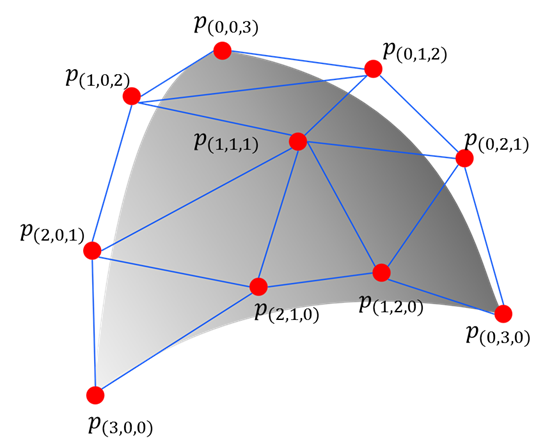
\includegraphics[width=0.75\hsize]{bezier-triangle.png}
    \caption{A B\'ezier simplex for $M = 3$, $D = 3$.}\label{fig:Bezier-simplex}
\end{figure}
We denote the set of non-negative integers (including zero!) by $\N$.
Let $M, D, L$ be arbitrary integers in $\N$ and $\N_D^M := \set{(d_1, \dots, d_M) \in \N^M | \sum_{m = 1}^M d_m = D}$.
As shown in \Cref{fig:Bezier-simplex}, an \emph{$(M - 1)$-B\'ezier simplex of degree $D$} is a mapping $\bm b: \Delta^{M - 1} \to \R^L$ determined by \emph{control points} $\bm p_{\bm d} \in \R^L$ $(\bm d \in \N_D^M)$ as follows:
\begin{equation}\label{eqn:bezier-simplex}
    \bm b(\bm t) := \sum_{\bm d \in \N_D^M} \binom{D}{\bm d} \bm t^{\bm d} \bm p_{\bm d}
\end{equation}
where $\binom{D}{\bm d} := \frac{D!}{d_1! d_2! \cdots d_M!}$ is a multinomial coefficient, and $\bm t^{\bm d} := t^{d_1}_1 t^{d_2}_2 \cdots t^{d_M}_M$ is a monomial (not vector) for each $\bm t := (t_1, \dots, t_M) \in \Delta^{M - 1}$ and $\bm d := (d_1, \dots, d_M) \in \N^M_D$.

\cite{Kobayashi2019} proposed two B\'ezier simplex fitting algorithms: the all-at-once fitting and the inductive skeleton fitting.
They are different in not an only fitting algorithm but also sampling strategy.
The all-at-once fitting requires a training set $S_N:=\set{(\bm t_n, \bm x_n) \in \Delta^{M - 1} \times \R^L | n = 1, \dots, N}$ and adjusts all control points at once by minimizing the OLS loss: $\frac{1}{N}\sum_{n = 1}^N \norm{\bm x_n - \bm b(\bm t_n)}^2$.

The inductive skeleton fitting, on the other hand, requires skeleton-wise sampled training sets $S_{N^{(m)}} := \set{(\bm t^{(m)}_n, \bm x^{(m)}_n) \in \Delta^{(m)} \times \R^L | n = 1, \dots, N^{(m)}}~(m = 0, \dots, M - 1)$.
It also divides control points as $\bm p_{\bm d^{(m)}}$ such that $\bm d^{(m)}$ has exactly $m + 1$ non-zero elements.
Such $\bm p_{\bm d^{(m)}}$ determines the $m$-skeleton of a B\'ezier simplex.
The inductive skeleton fitting inductively adjusts $\bm p_{\bm d^{(m)}}$ from $m = 0$ to $M - 1$ by minimizing the OLS loss of the $m$-skeleton $\frac{1}{N^{(m)}}\sum_{n=1}^{N^{(m)}} \norm{\bm x^{(m)}_n - \bm b(\bm t_n^{(m)})}^2$.


%%%%%%%%%%%%%%%%%%%%%%%%%%%%%%%%%%%%%%%%%%%%%%%%%%%%%%%%%%%%%%%%%%%%%%%%%%%%%%%%
\subsection{The \texorpdfstring{$\ell_2$}{l2}-risk}
In this paper, we consider the following fitting problem: As \Cref{fig:sampling} illustrates, a sample point $(\bm t, \bm x)\in \Delta^{M - 1} \times \R^L$ is taken from an unknown B\'ezier simplex $\bm b: \Delta^{M - 1} \to \R^L$ with additive Gaussian noise $\bm \varepsilon \sim N(\bm 0, \sigma^2 \bm I)$, that is, $\bm x = \bm b(\bm t) + \bm \varepsilon$.
For the all-at-once fitting, $S_N = \set{(\bm t_n, \bm x_n)}$ follows the uniform distribution on the domain of the B\'ezier simplex: $\bm t_n \sim U(\Delta^{M - 1})$ and $\bm x_n = \bm b(\bm t_n) + \bm \varepsilon_n$.
For the inductive skeleton fitting, $S_{N^{(m)}} = \set{(\bm t_n^{(m)}, \bm x_n^{(m)})}$ follows the uniform distribution on the $m$-skeleton of the domain of the B\'ezier simplex: $\bm t_n^{(m)} \sim U(\Delta^{(m)})$ and $\bm x_n^{(m)} = \bm b(\bm t_n^{(m)}) + \bm \varepsilon_n^{(m)}$.
A B\'ezier simplex estimated from $S_N$ is denoted by $\bm{\hat b}(\bm t | S_N)$.
For both method, we asymptotically evaluate the $\ell_2$-risk below as $N \to \infty$.
\begin{equation}\label{def:risk}
    R_N := \E_{S_N}\sqbra{\E_{\bm t \sim U(\Delta^{M - 1})} \norm{\bm b(\bm t) - \hat{\bm b}(\bm t | S_N)}^2}.
\end{equation}
For the inductive skeleton fitting, we put $S_N = S_{N^{(0)}} \cup \dots \cup S_{N^{(M - 1)}}$ subject to $N = N^{(0)} + \dots + N^{(M - 1)}$.

\begin{figure}[ht]
    \centering
    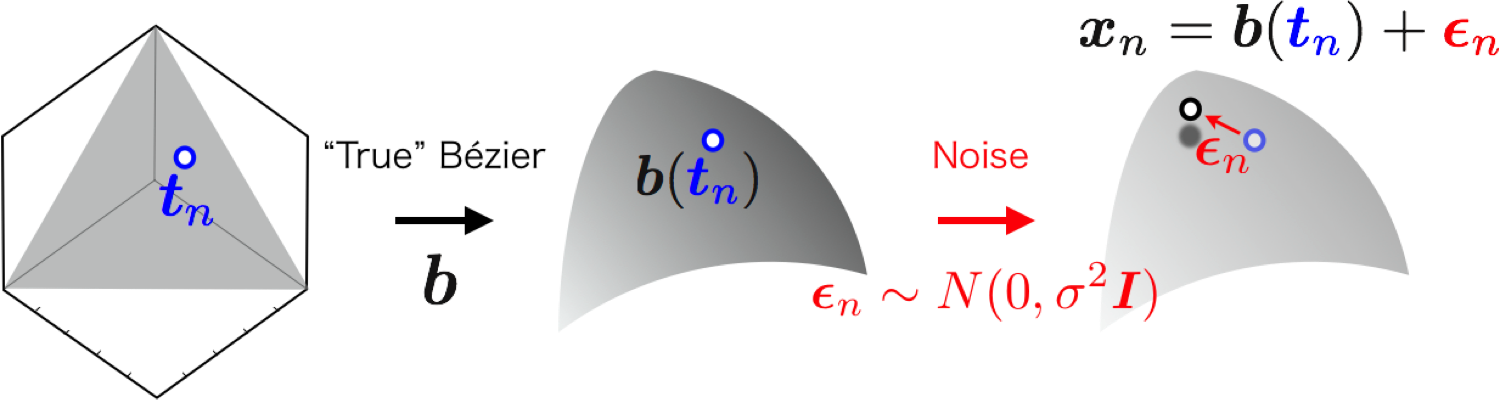
\includegraphics[width=1\hsize]{sampling.png}
    \caption{An illustration of taking a sample point on the true B\'ezier simplex with additive noise.}\label{fig:sampling}
\end{figure}


%%%%%%%%%%%%%%%%%%%%%%%%%%%%%%%%%%%%%%%%%%%%%%%%%%%%%%%%%%%%%%%%%%%%%%%%%%%%%%%%
\section{Asymptotic risk of B\'ezier simplex fitting}\label{sec:asymptotic-risk}
Let us first focus on the fact: the subtraction inside the $\ell_2$-norm in \cref{def:risk} can be also written as a B\'ezier simplex:
\begin{align}
    \bm b(\bm t) - \hat{\bm b}(\bm t | S_N)
    =
    \sum_{A = 1}^{\card{\N_D^M}}
    \binom{D}{\bm d_A} \bm t^{\bm d_A}
    \bm p'_{\bm d_A}.
    \label{def:subt}
\end{align}
Each $A$-th control point $\bm p_{\bm d_A}'$ of this B\'ezier simplex is defined by difference between the target control point $\bm p_{\bm d_A}$ and the model control point $\hat{\bm p_{\bm d_A}}(S_N)$, i.e.~$\bm p'_{\bm d_A} = \bm p_{\bm d_A} - \hat{\bm p}_{\bm d_A}(S_N)$.
To simplify the summation notation, we introduce a size $\card{\N_D^M} \times L$ matrix $\bm P$ composed by the $l$-th element of the $A$-th control point and a column vector $\bm z$:
\begin{align}
    (\bm P)_{Al} = (\bm p_{\bm d_A}')_l, \
    \bm z^\top =
    \Big[
        \binom{D}{\bm d_1} \bm t^{\bm d_1},
        \dots,
        \binom{D}{\bm d_{\card{\N_D^M}}} \bm t^{\bm d_{\card{\N_D^M}}}
    \Big].
    \label{def:Pz}
\end{align}
Note that $\bm t^{\bm d} = t_1^{d_1} t_2^{d_2} \cdots t_M^{d_M}$ is scalar, and $\bm z$ is a vector.
Then, the B\'ezier simplex \cref{def:subt} can be represented by column vector $\bm P^\top \bm z$, and its squared norm is equal to $\norm{\bm P^\top \bm z}^2 = \bm z^\top \bm P \bm P^\top \bm z$, or $\sum_{A, B}z_A z_B (\bm P \bm P^\top )_{AB}$ in component.
The risk \cref{def:risk} is defined by an expectation value of this norm.
$\E_{\bm t}$ only acts to $\bm z$ and $\E_{S_N}$ only acts to $\bm P$.
Therefore, we arrive at
\begin{align}
    R_N
    =
    \sum_{\bm d_A, \bm d_B \in \N_D^M}
    \ZZ_{AB}
    \E_{S_N} \sqbra{({\bm P} {\bm P}^\top)_{AB}},
    \label{eqn:risk}
\end{align}
where
\begin{align}
    \Sigma_{AB}
    =
    \E_{\bm t}[z_A z_B]
    =
    \binom{D}{\bm d_A}
    \binom{D}{\bm d_B}
    \E_{\bm t}[\bm t^{\bm d_A + \bm d_B}].
    \label{def:sigmaexp}
\end{align}
We can get closed form of $\ZZ_{AB}$ by performing integral $\E_{\bm t}$ explicitly.
The following theorem provides the result.
\begin{theorem}\label{thm:risk}
The matrix element $\ZZ_{AB}$ is calculated by
\begin{align}
    \ZZ_{AB} =
        \binom{2D + M - 1}{M - 1}^{-1}
        \binom{D}{\bm d_A} \!
        \binom{D}{\bm d_B} \!
        \binom{2D}{\bm d_A + \bm d_B}^{-1}
        \label{eqn:ZZ-def}
\end{align}
\end{theorem}
The proof is provided in the supplementary materials. %\cref{apnd:sec:proof-of-main-theorem}
\footnote{A longer version of this paper including appendix is available at \url{https://arxiv.org/abs/1906.06924}}%)
.
The equation \cref{eqn:risk} means that the asymptotic value of the risk function depends only on a choice of the matrix $\bm P$.


%%%%%%%%%%%%%%%%%%%%%%%%%%%%%%%%%%%%%%%%%%%%%%%%%%%%%%%%%%%%%%%%%%%%%%%%%%%%%%%%
\subsection{All-at-once fitting}\label{sec:all-at-once-fitting}
The matrix $\bm P$ determined by the all-at-once fitting algorithm, $\bm P_\mathrm{AAO}$, is minimizing the OLS loss:
\begin{align}
    \frac{1}{N} \sum_{n = 1}^N \Big\| \underbrace{\bm b(\bm t_n) + \bm \varepsilon_n}_{\bm x_n}  - \hat{\bm b}(\bm t_n) \Big\|^2
    &= \frac{1}{N} \sum_{n = 1}^N \norm{\bm P^\top \bm z_n + \bm \varepsilon_n}^2 \notag \\
    &= \frac 1 N \norm{\bm Z \bm P + \bm Y}_{\mathrm F}^2, \label{eqn:rss}
\end{align}
where $\norm{\cdot}_\mathrm{F}$ is the Frobenius norm.
Here, we introduced an $N \times \card{\N_D^M}$ matrix $\bm Z$ and an $N \times L$ matrix $\bm Y$:
\begin{align}
    \bm Z = \sqbra{\bm z_1 \bm z_2 \cdots \bm z_N}^\top,\ 
    \bm Y = \sqbra{\bm \varepsilon_1 \bm \varepsilon_2 \cdots \bm \varepsilon_N}^\top.
\end{align}
Minimizing \cref{eqn:rss} is a traditional problem and we get $\bm P_\mathrm{AAO} = -\paren{\bm Z^\top \bm Z}^{-1}\bm Z^\top \bm Y$.
Note that $\bm Z$ includes $N$ sample points on $\Delta^{M - 1}$ and $\bm Y$ is a set of $N$ noises on $\R^L$.
These are all independent, so the expectation $\E_{S_N}$ can be factorized to $\E_{\bm Z} \E_{\bm Y}$.


%%%%%%%%%%%%%%%%%%%%%%%%%%%%%%%%%%%%%%%%%%%%%%%%%%%%%%%%%%%%%%%%%%%%%%%%%%%%%%%%
\paragraph{Calculation of the asymptotics}
We need to calculate the expectation value of the matrix $\bm P_\mathrm{AAO} \bm P_\mathrm{AAO}^\top = \paren{\bm Z^\top \bm Z}^{-1}\bm Z^\top \bm Y \bm Y^\top \bm Z \paren{\bm Z^\top \bm Z}^{-1}$ over $\bm Z$ and $\bm Y$.
As easily checked, $\E_{\bm Y}[\bm Y \bm Y^\top] = \sigma^2 L \bm I_{N \times N}$, so we get
\begin{align}
    \E_{S_N} \sqbra{\bm P_\mathrm{AAO} \bm P_\mathrm{AAO}^\top}
    &=
    \sigma^2 L \cdot \E_{\bm Z} \sqbra{\paren{\bm Z^\top \bm Z}^{-1}}
    .
    \label{eqn:P_AAO-P_AAO}
\end{align}
Now, the matrix $(\bm Z^\top \bm Z)$ is an average over the sample:
\begin{align}
    \frac{1}{N}
    \paren{\bm Z^\top \bm Z}_{AB}
    =
    \binom{D}{\bm d_A}
    \binom{D}{\bm d_B}
    \sum_{n = 1}^N
    \frac{1}{N}
    \bm t_n^{\bm d_A + \bm d_B}
    ,
\end{align}
and it converges to the matrix $\ZZ_{AB} $ defined in \cref{def:sigmaexp} and \cref{eqn:ZZ-def} as $N \to \infty$ by using the law of large numbers: $\paren{\bm Z^\top \bm Z}_{AB} \overset{p}{\to} N \ZZ_{AB}$.
To substitute it to \cref{eqn:P_AAO-P_AAO}, however, we need to guarantee $\ZZ_{AB}$ has the inverse matrix.
We can show it by the following theorem.
\begin{theorem}\label{thm:sigma-is-non-singular}
Let $V_{M, D}$ be a vector space spanned by
\[
    Z = \Set{\frac{\bm{t}^{\bm{d}}}{\bm{d}!} | \bm{d} = (d_1, \dots, d_M) \in \N^M_D}.
\]
Then the map
\[
    \begin{array}{ccc}
    L:V_{M, D} \times V_{M, D} & \longrightarrow & \R\\
    \ \ \ \  \rotatebox{90}{$\in$}    &                 & \rotatebox{90}{$\in$} \\
    \ \ \ \  (P, Q)                   & \longmapsto     & \int_{\Delta^{M - 1}} P(\bm{t}) Q(\bm{t}) d\bm{t}
    \end{array},
\]
is a non-degenerate bilinear form.
Moreover, the matrix corresponding to this bilinear form is $\Sigma_{AB}$ in \cref{eqn:ZZ-def}.
In particular, for any $D, M$, the matrix $\ZZ_{AB}$ is non-singular.
\end{theorem}
The precise proof is given in the supplementary materials. %(\cref{apnd:sec:proof-of-regularity})
In summary, our formula for the asymptotic form of the risk for the all-at-once fitting is
\begin{align*}
    R_N
    \overset{p}{\to}
    \frac{\sigma^2 L}{N} \sum_{A, B} \ZZ_{AB} \ZZ^{-1}_{AB}
    =
    \frac{\sigma^2 L}{N} \binom{D + M - 1}{D} \quad (N \to \infty).
\end{align*}
We can further simplify the result by using: $\sum_{AB} \ZZ_{AB} \ZZ^{-1}_{AB} = \card{\N_D^M} = \binom{D + M - 1}{D}$, which is relatively easy to show (see the supplementary materials).


%%%%%%%%%%%%%%%%%%%%%%%%%%%%%%%%%%%%%%%%%%%%%%%%%%%%%%%%%%%%%%%%%%%%%%%%%%%%%%%%
\subsection{Inductive skeleton fitting}\label{sec:inductive-skeleton-fitting}
So far, we did not take any explicit order of the control point indices $A$.
From now on, let us take a specific order
\begin{align}
    \bm P^\top = [{\bm P^{(0)}}^\top {\bm P^{(1)}}^\top \cdots {\bm P^{(M - 1)}}^\top ],
\end{align}
where $\bm P^{(m)}$ is the submatrix of $\bm P$ composed by control points on $\Delta^{(m)}$.
Similarly, we introduce an order of control point indices $\bm d_A$ as follows:
\begin{align*}
    [
    \bm d_1^{(0)}, \dots, \bm d_{n_0}^{(0)},
    \bm d_1^{(1)}, \dots, \bm d_{n_1}^{(1)},
    \dots,
    \bm d_1^{(M - 1)}, \dots, \bm d_{n_{M - 1}}^{(M - 1)}
    ],
\end{align*}
where $\bm d^{(m)}_n$ is the $n$-th index of control points on the $m$-skeleton and $n_m$ is the number of control points on the $m$-skeleton.
The inductive skeleton fitting is described by an inductive procedure of determining control points matrices $\bm P^{(m)}$ from low $m = 0, 1, \dots, M - 1$.
That is, first it fits the vertices of a B\'ezier simplex by moving the control points of the lowest dimension ($\bm P^{(0)}$); then, it fits the edges by moving the control points of the second lowest dimension ($\bm P^{(1)}$); this process goes on with increasing dimensions and finishes at the highest dimension ($\bm P^{(M - 1)}$).
In the $m$-th step, sample points $\bm t^{(m)}$ on $\Delta^{(m)}$ are given.
The corresponding $\bm z^{(m)}$ defined in \cref{def:Pz} has the following form:
\begin{align*}
    &{\bm z^{(m)}}^\top
    =
    [
    {\bm z^{(m) [0]}}^\top
    {\bm z^{(m) [1]}}^\top
    \cdots
    {\bm z^{(m) [m]}}^\top
    \bm 0
    \cdots
    \bm 0
    ], \text{where}
    \\
    &
    {\bm z^{(m) [k]}}^\top
    =
    \sqbra{
    \binom{D}{\bm d_1^{(k)}}
    (\bm t^{(m)})^{\bm d_1^{(k)}}
    , \dots,
    \binom{D}{\bm d_{n_k}^{(k)}}
    (\bm t^{(m)})^{\bm d_{n_k}^{(k)}}
    },
\end{align*}
because $(\bm t^{(m)})^{\bm d^{(k>m)}}$ includes $0^{d_\bullet^{(k)}\neq 0} = 0$ by definition.
Thanks to these zeros, the OLS loss reduces as follows:
\begin{align}
    &
    \sum_{n = 1}^{N^{(m)}}
    \norm{
    (\bm P^{(m)})^T \bm z_n^{(m) [m]}
    +
    \sum_{k<m}
    (\bm P^{(k)})^T \bm z_n^{(m) [k]}
    +
    \bm \varepsilon_n^{(m)}
    }^2
    \notag \\
    &=
    \norm{\bm Z^{(m) [m]} \bm P^{(m)} + \sum_{k < m} \bm Z^{(m) [k]} \bm P^{(k)} + \bm Y^{(m)}}_\mathrm{F}.
    \label{eqn:OLS}
\end{align}
Each matrix is defined as follows.
\begin{align*}
    {\bm Z}^{(m) [k]}
    &=
    \sqbra{{\bm z}_1^{(m) [k]}
    \cdots
    {\bm z}_{N^{(m)}}^{(m) [k]}}^\top,
    {\bm Y}^{(m)}
    =
    \sqbra{{\bm \varepsilon}_1^{(m)}
    \cdots
    {\bm \varepsilon}_{N^{(m)}}^{(m)}}^\top.
\end{align*}
In addition, we regard lower-dimensional control points already fixed, so the net objective control points are ones included in $\bm P^{(m)}$.
By repeating similar procedure done in the all-at-once fitting, we can conclude $\bm P^{(m)}$ is determined as
\begin{equation}
    \begin{split}
    {\bm P}_\mathrm{ISK}^{(m)}
    =
    -
    &[({\bm Z}^{(m)})^\top {\bm Z}^{(m)}]^{-1}
    ({\bm Z}^{(m)})^\top \\
    \times &\paren{
    {\bm Y}^{(m)}
    +
    \sum_{k < m}
    {\bm Z}^{(m) [k]}
    {\bm P}_\mathrm{ISK}^{(k)}
    }
    \label{eqn:P_OLS}
    \end{split}
\end{equation}


%%%%%%%%%%%%%%%%%%%%%%%%%%%%%%%%%%%%%%%%%%%%%%%%%%%%%%%%%%%%%%%%%%%%%%%%%%%%%%%%
\paragraph{Calculation of the asymptotics}
From this expression, we get ${\bm P_\mathrm{ISK}} {\bm P_\mathrm{ISK}}^\top = \oplus_{i, j = 0}^{M - 1} {\bm P}^{(i)}_\mathrm{ISK} ({\bm P}^{(j)}_\mathrm{ISK})^\top$.
The expected value of each $(i, j)$-term is needed to evaluate the risk \cref{eqn:risk}.
The following theorem provides us an algorithm to asymptotically calculate the expectation.
\begin{theorem}
Let $I_{\bm d} = \set{i | d_i \neq 0} \subseteq \Set{1, \dots, M}$ and $\bm \Lambda^{(m) [k]}$ be an $n_m \times n_k$ matrix defined by
\begin{align}
    &({\bm \Lambda}^{(m) [k]})_{ \bm d ^{(m)} \bm d ^{(k)} }
    =
    1_{I_{\bm d^{(m)}}\supseteq I_{\bm d^{(k)}}}
    \binom{M}{m + 1}^{-1}
    \ZZ^{(m)}_{\bm d^{(m)} \bm d^{(k)}}
    , \notag
    \\
    &
    \text{where }
    \ZZ_{\bm d_A \bm d_B}^{(m)}
    :=
    \binom{2D + m}{m}^{-1}
    \binom{D}{\bm d_A}
    \binom{D}{\bm d_B}
    \binom{2D}{\bm d_A + \bm d_B}^{-1},
    \notag
\end{align}
and $1_{X} = 1$ if $X$ is true, otherwise 0.
Then we get the asymptotic submatrix $\bm X^{(i)(j)}$
\begin{multline}
    \E_{S_N}
    \sqbra{
    {\bm P}^{(i)}_\mathrm{ISK}
    ({\bm P}^{(j)}_\mathrm{ISK})^\top
    }
    \overset{p}{\to} \bm X^{(i)(j)}:=
    \\
    \sigma^2 L
    \sum_{
    \substack{
    m \leq i
    \\
    m \leq j
    }}
    \sum_{
    \substack{
    m \leq k_1 < \dots < k_{\heartsuit} < i
    \\
    m \leq l_1 < \dots < l_{\spadesuit} < j
    }
    }
    \frac{(-1)^{\heartsuit + \spadesuit}}{N^{(m)}}
    {\bm \Lambda}_{\heartsuit}
    \bm \Lambda_{(m)}
    {\bm \Lambda}_{\spadesuit}
    \label{eqn:P_OLS-P_OLS}
\end{multline}
where the summation runs for all possible increasing sequences $[k_1, \dots, k_\heartsuit]$ and $[l_1, \dots, l_\spadesuit]$, and
\begin{align}
    &{\bm \Lambda}_{\heartsuit}=
    {\bm \Lambda}_{(i)}
    {\bm \Lambda}^{(i) [k_{\heartsuit}]}
    {\bm \Lambda}_{(k_{\heartsuit})}
    \cdots
    {\bm \Lambda}^{(k_1) [m]}
    ,\notag\\
    &{\bm \Lambda}_{\spadesuit}=
    {\bm \Lambda}^{[m](l_1)}
    \cdots
    {\bm \Lambda}_{(l_{\spadesuit})}
    {\bm \Lambda}^{[l_{\spadesuit}](j)}
    {\bm \Lambda}_{(j)}
    ,\notag \\
    &{\bm \Lambda}^{[k](m)}
    =
    ({\bm \Lambda}^{(m) [k]})^\top,
    \quad
    {\bm \Lambda}_{(m)}
    =
    ({\bm \Lambda}^{(m) [m]})^{-1}
    .
    \label{eqn:Lamb}
\end{align}
\end{theorem}
For the complete derivation, see the supplementary materials.
The asymptotic form of the risk for the inductive skeleton fitting is, therefore, calculated by
\begin{align}
    &R_{N^{(0)}, \dots, N^{(M - 1)}}
    =
    \sum_{\bm d_A, \bm d_B \in \N_D^M}
    \ZZ_{AB}
    \Big(
    \bigoplus_{i, j = 0}^{M - 1}
    \bm X^{(i)(j)}
    \Big)_{AB}
    \notag
    .
\end{align}
We found a candidate of closed-form with $M = 2$ risks as $(D - 1) / N^{(1)} + 4 / D(D + 2)N^{(0)}$, but postpone deriving the closed-form of it for arbitrary $(D, M)$ for future work.
Instead, we show numerically computed risks in \cref{tab:risk-inductive}.

\begin{table}[ht]
    \centering
    \footnotesize
    \caption{Numerically computed asymptotic risks of the inductive skeleton fitting $R_{N^{(0)}, \dots, N^{(M - 1)}}$ ($M$: the dimension of the B\'ezier simplex, $D$: the degree of the B\'ezier simplex, $N^{(m)}$: the sample size for the $m$-skeleton).}\label{tab:risk-inductive}
    {\tabcolsep = 1mm
    \begin{tabular}{crr}
    \toprule
    $M$ &
    \multicolumn{1}{c}{$D = 2$} &
    \multicolumn{1}{c}{$D = 3$}
    \\
    \midrule
    $2$ &
    $\displaystyle\frac{1.00}{N^{(1)}} + \frac{0.50}{N^{(0)}}$ &
    $\displaystyle\frac{2.00}{N^{(1)}} + \frac{0.27}{N^{(0)}}$
    \\[6pt]
    $3$ &
    $\displaystyle\frac{3.00}{N^{(1)}} + \frac{0.38}{N^{(0)}}$ &
    $\displaystyle\frac{1.00}{N^{(2)}} + \frac{3.54}{N^{(1)}} + \frac{0.15}{N^{(0)}}$
    \\[6pt]
    $4$ &
    $\displaystyle\frac{5.14}{N^{(1)}} + \frac{0.46}{N^{(0)}}$ &
    $\displaystyle\frac{5.33}{N^{(2)}} + \frac{4.70}{N^{(1)}} + \frac{0.17}{N^{(0)}}$
    \\[6pt]
    $5$ &
    $\displaystyle\frac{7.14}{N^{(1)}} + \frac{0.64}{N^{(0)}}$ &
    $\displaystyle\frac{13.33}{N^{(2)}} + \frac{6.67}{N^{(1)}} + \frac{0.21}{N^{(0)}}$
    \\[6pt]
    $6$ &
    $\displaystyle\frac{8.93}{N^{(1)}} + \frac{0.82}{N^{(0)}}$ &
    $\displaystyle\frac{24.24}{N^{(2)}} + \frac{9.74}{N^{(1)}} + \frac{0.26}{N^{(0)}}$
    \\[6pt]
    $7$ &
    $\displaystyle\frac{10.50}{N^{(1)}} + \frac{1.02}{N^{(0)}}$ &
    $\displaystyle\frac{37.10}{N^{(2)}} + \frac{13.84}{N^{(1)}} + \frac{0.31}{N^{(0)}}$
    \\[6pt]
    $8$ &
    $\displaystyle\frac{11.87}{N^{(1)}} + \frac{1.21}{N^{(0)}}$ &
    $\displaystyle\frac{51.17}{N^{(2)}} + \frac{18.73}{N^{(1)}} + \frac{0.37}{N^{(0)}}$
    \\
    \bottomrule
    \end{tabular}
    }
\end{table}


%%%%%%%%%%%%%%%%%%%%%%%%%%%%%%%%%%%%%%%%%%%%%%%%%%%%%%%%%%%%%%%%%%%%%%%%%%%%%%%%
\subsection{All-at-once vs.\ Inductive skeleton}\label{sec:all-vs-inductive}
Given a total sample size $N$, we can minimize the ISK-risk by finding the optimally-decoupled subsample sizes:
\begin{equation}
    R_N := \min_{
    \substack{N^{(0)}, \dots, N^{(M - 1)}
    \\
    N = N^{(0)} + \dots + N^{(M - 1)}
    }} \Set{R_{N^{(0)}, \dots, N^{(M - 1)}}} .
\end{equation}
We calculated optimal risks for all cases shown in \cref{tab:risk-inductive} and compared them to the risks of the all-at-once fitting.
\Cref{tab:risk-comparison} shows the results.
\begin{table}[H]
    \small
    \centering
    \caption{Comparison of asymptotic risks of the all-at-once $R_N^\mathrm{AAO}$ vs.\ the inductive skeleton with the optimal subsample ratio $R_N^\mathrm{ISK}$ ($M$: the dimension of the B\'ezier simplex, $D$: the degree of the B\'ezier simplex, $N$: the sample size). The winner is shown in bold.}\label{tab:risk-comparison}
    \begin{tabular}{l|rr|rr}
    \toprule
    & \multicolumn{2}{c|}{$D = 2$} & \multicolumn{2}{c}{$D = 3$} \\
    & $R_{N}^\mathrm{AAO}$ & $R_N^\mathrm{ISK}$
    & $R_{N}^\mathrm{AAO}$ & $R_N^\mathrm{ISK}$
    \\
    \midrule
    $M = 2$ &
    $3.0 / N$ &
    $\bm{2.91} / N$ &
    $4.0 / N$ &
    $\bm{3.73} / N$
    \\
    $M = 3$ &
    $6.0 / N$ &
    $\bm{5.50} / N$ &
    $\bm{10.0} / N$ &
    $10.650 / N$
    \\
    $M = 4$ &
    $10.0 / N$ &
    $\bm{8.67} / N$ &
    $\bm{20.0} / N$ &
    $23.88 / N$
    \\
    $M = 5$ &
    $15.0 / N$ &
    $\bm{11.99} / N$ &
    $\bm{35.0} / N$ &
    $44.76 / N$
    \\
    $M = 6$ &
    $21.0 / N$ &
    $\bm{15.17} / N$ &
    $\bm{56.0} / N$ &
    $73.14 / N$
    \\
    $M = 7$ &
    $28.0 / N$ &
    $\bm{18.07} / N$ &
    $\bm{84.0} / N$ &
    $107.57 / N$
    \\
    $M = 8$ &
    $36.0 / N$ &
    $\bm{20.68} / N$ &
    $\bm{120.0} / N$ &
    $146.21 / N$
    \\
    \bottomrule
    \end{tabular}
\end{table}

As one can see, the optimum inductive skeleton fitting outperforms the all-at-once fitting for $D = 2$, but it is not always true for $D = 3$.
On $D = 2$, in fact, we can show that the minimum value of the inductive skeleton always less than the asymptotic risk of the corresponding all-at-one fitting.


%%%%%%%%%%%%%%%%%%%%%%%%%%%%%%%%%%%%%%%%%%%%%%%%%%%%%%%%%%%%%%%%%%%%%%%%%%%%%%%%
\section{Numerical examples}\label{sec:numerical-examples}
We examine the empirical performances of the all-at-once fitting and the inductive skeleton fitting and verify the asymptotic risks derived in \cref{sec:all-at-once-fitting} over synthetic instances and multi-objective optimization instances.
Experiment programs were implemented in Python 3.7.1 and run on a Windows 7 PC with an Intel Core i7-4790CPU (3.60 GHz) and 16 GB RAM\footnote{The source code and library dependencies are provided in \url{https://github.com/rafcc/aaai-20.1534}.}.


%%%%%%%%%%%%%%%%%%%%%%%%%%%%%%%%%%%%%%%%%%%%%%%%%%%%%%%%%%%%%%%%%%%%%%%%%%%%%%%%
\subsection{Synthetic instances}\label{sec:synthetic-instances}
We consider the fitting problem where the true B\'ezier simplex $\bm b(\bm{t})~(\bm t \in \Delta^{M - 1})$ is an $(M - 1)$-dimensional unit simplex on $\R^L$, and randomly generate $N$ training points $\set{(\bm t_n, \bm x_n)}_{n = 1}^N$ as $\bm x_n = \bm b(\bm t_n) + \bm{\varepsilon}_n~(\bm \varepsilon_n \sim N(\bm 0, 0.1^2 \bm I))$.
This synthetic instance is parameterized by a tuple $(L, M, N)$.
The detailed data generation processes are shown in the supplementary materials. %(\cref{apnd:sec:numerical-experiments}).

In this experiment, we estimated the B\'ezier simplex with degree $D = 2$ or 3, and compared the following three fitting methods:
\begin{description}
    \item[all-at-once] the all-at-once fitting (\cref{sec:all-at-once-fitting});
    \item[inductive skeleton (non-optimal)] the inductive skeleton fitting (\cref{sec:inductive-skeleton-fitting}) with $N^{(0)} = \dots = N^{(M - 1)} = N / M$, which does not provide the optimal value of the risk shown in \cref{tab:risk-inductive};
    \item[inductive skeleton (optimal)] the inductive skeleton fitting (\cref{sec:inductive-skeleton-fitting}) where $N^{(0)}, \dots, N^{(M - 1)}$ are determined by minimizing the risk shown in \cref{tab:risk-inductive} under the constraints $\sum_{m = 0}^{M - 1} N^{(m)} = N$ and $N^{(m)}\geq 0~(m = 0, \dots, M - 1)$. The actual sample size $N^{(m)}$ for each $(D, M)$ are shown in the supplementary materials.%\cref{apnd:sec:numerical-experiments} (\cref{apnd:tab:optimal-subsample-ratio}).
\end{description}
When we calculated an approximation of the expected risk for each method, we randomly chose other 10000 parameters $\set{\bm{\hat t}_n}_{n = 1}^{10000}$ from $U(\Delta^{M - 1})$ as a test set and measured the mean squared error, $\mathrm{MSE} := \frac{1}{10000} \sum_{n = 1}^{10000} \norm{\bm b(\bm{\hat{t}}_n) - \bm{\hat{b}}(\bm{\hat{t}}_n)}^2$, where $\bm{\hat{b}}$ is the estimated B\'ezier simplex.
This experiment was conducted with the following tuple $(L, M, N)$ to observe how the empirical MSEs depend on $L, M$ and $N$ respectively:
\begin{itemize}
    \item $N \in \set{250, 500, 1000, 2000}$ with $(L, M) = (100, 8)$,
    \item $M \in \set{3,4,5,6,7,8}$ with $(L, N) = (100, 1000)$,
    \item $L \in \set{8, 25, 50, 100}$ with $(M, N) = (8, 1000)$,
\end{itemize}
For each $(L, M, N)$ with $D \in \set{2, 3}$, we ran 20 trials and measured MSEs.

Owing to space limitation, we only present typical results here. The remaining results are provided in the supplementary materials.
\Cref{fig:MSE-vs-N} shows box plots of MSEs over 20 trials and our theoretical risks \cref{eqn:risk} and \cref{tab:risk-inductive} for each $N \in \set{250, 500, 1000, 2000}$ with $(L, M) = (100, 8)$ and $D \in \set{2, 3}$.
We observe that these figures empirically show that our theoretical risks are correct for both $D = 2$ and 3, and the gaps between the MSEs and the risks are sufficiently small at $N = 1000$.
For both $D = 2$ and 3, the inductive skeleton (optimal) always achieved lower MSEs than that of the inductive skeleton (non-optimal).
This result suggests the effectiveness of minimizing the risk (\cref{tab:risk-comparison}) with respect to the sample size of each skeleton.
In addition, the inductive skeleton fitting (optimal) also outperformed the all-at-once fitting in the case of $D = 2$.
This result also supports the discussion described in \cref{sec:all-vs-inductive}.

\begin{figure*}[t]
    \centering
    \subfloat[$D=2$]{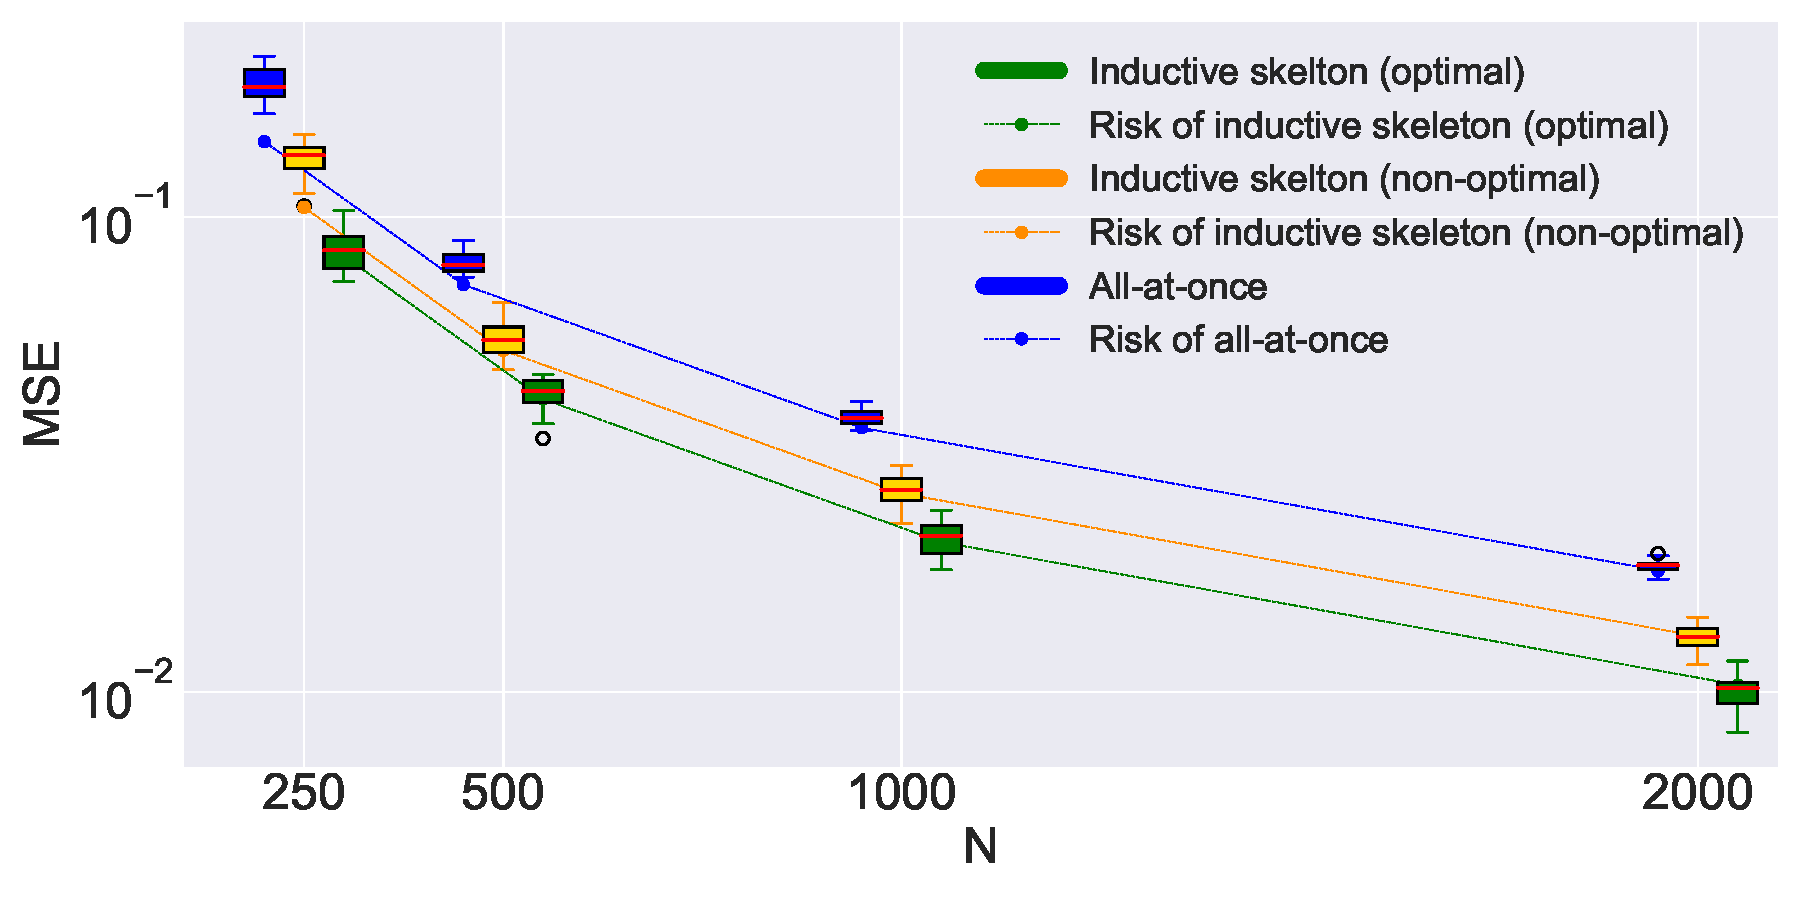
\includegraphics[width=0.5\hsize]{D=2_M=8_L=100.pdf}\label{fig:MSE-vs-N-D=2}}
    \subfloat[$D=3$]{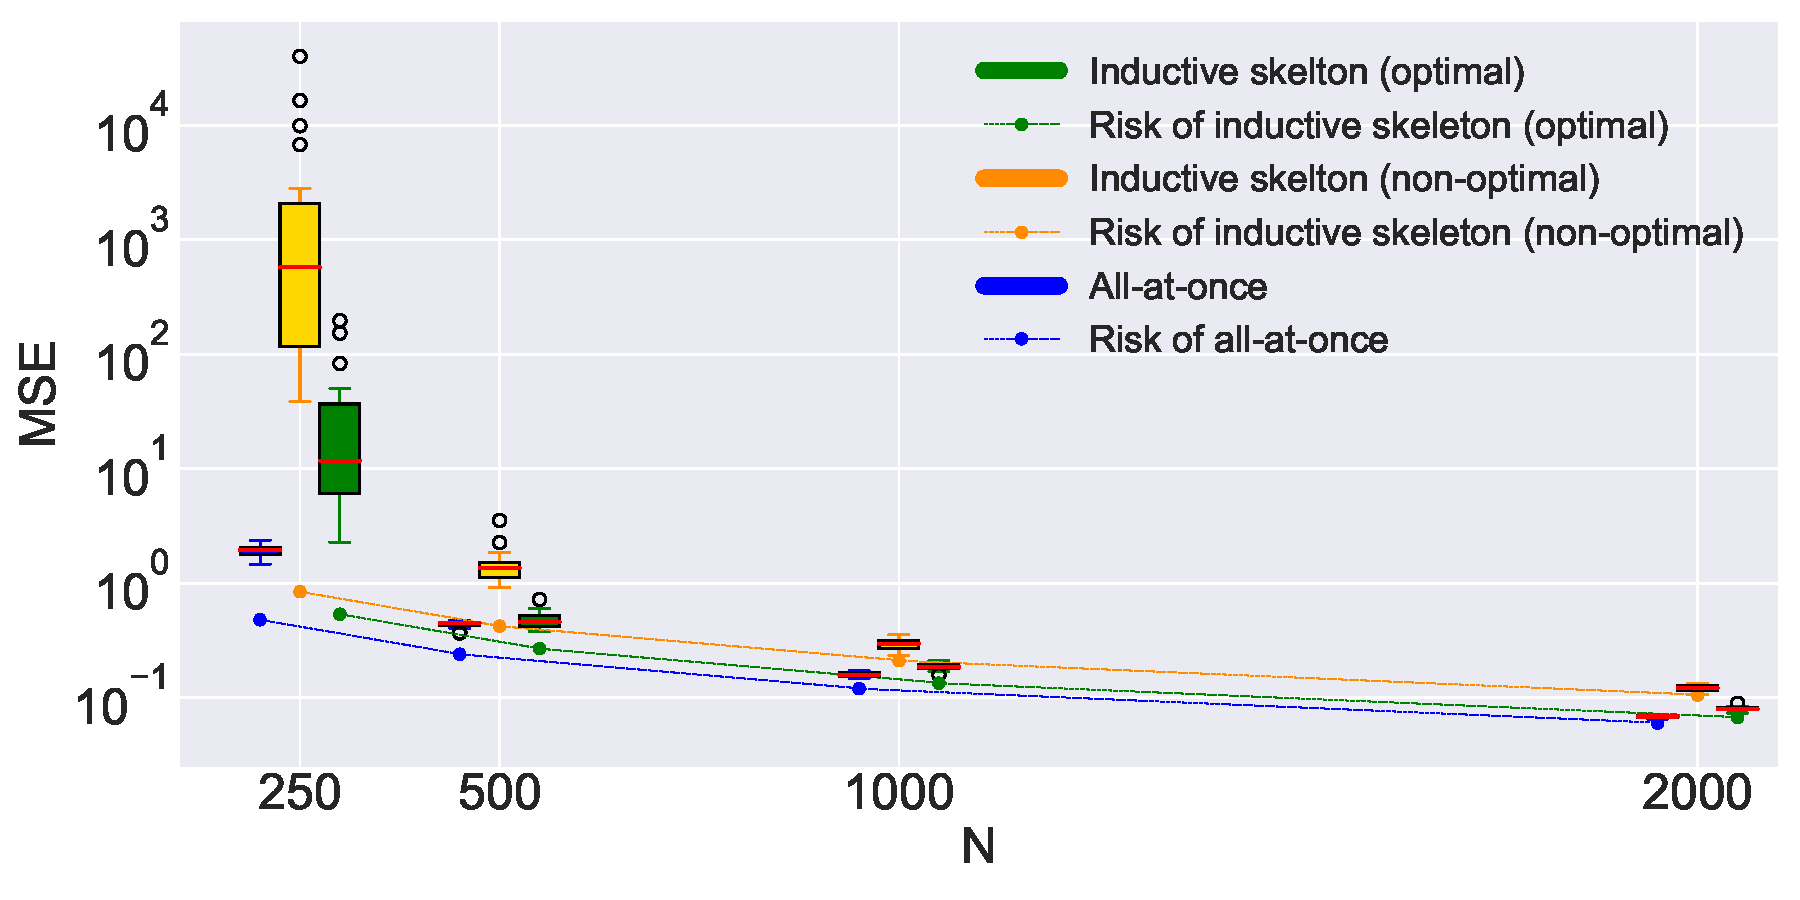
\includegraphics[width=0.5\hsize]{D=3_M=8_L=100.pdf}\label{fig:MSE-vs-N-D=3}}
    \caption{Sample size $N$ vs.\ MSE with $(L, M) = (100, 8)$ (boxplots: empirical MSEs over 20 trials, lines: theoretical risks).}
    \label{fig:MSE-vs-N}
\end{figure*}


%%%%%%%%%%%%%%%%%%%%%%%%%%%%%%%%%%%%%%%%%%%%%%%%%%%%%%%%%%%%%%%%%%%%%%%%%%%%%%%%
\subsection{Multi-objective optimization instances}\label{sec:MOP-instances}
\begin{table*}[t]
    \caption{MSE (avg.\ $\pm$ s.d.\ over 20 trials) for the Pareto sets of the location problem and the group lasso. The winners with significance level $p < 0.05$ are shown in bold.}
    \label{tab:MSE-MOP-instances-pareto-set}
    \centering
    \subfloat[Location problem]{
        \small
        {\tabcolsep = 1mm
        \begin{tabular}{crcc}
        \toprule
        $D$&$N$ & \multicolumn{1}{c}{All-at-once} & \multicolumn{1}{c}{Inductive-skeleton (optimal)}\\
        \midrule
        2 & 250      &1.0246e+00 $\pm$ 1.7031e-03      &\textbf{1.0227e+00 $\pm$ 2.3045e-03} \\
          & 500      &1.0119e+00 $\pm$ 5.3916e-04      &\textbf{1.0108e+00 $\pm$ 7.5912e-04} \\
          & 1000     &1.0060e+00 $\pm$ 2.6182e-04      &\textbf{1.0055e+00 $\pm$ 4.7063e-04} \\
          & 2000     &1.0029e+00 $\pm$ 1.8406e-04      &1.0028e+00 $\pm$ 2.7489e-04 \\
        \midrule
        3 & 250      &\textbf{1.0430e+00 $\pm$ 3.3097e-03}      &1.0458e+00 $\pm$ 4.4068e-03 \\
          & 500      &\textbf{1.0203e+00 $\pm$ 1.1845e-03}      &1.0219e+00 $\pm$ 1.4369e-03 \\
          & 1000     &\textbf{1.0100e+00 $\pm$ 3.9162e-04}      &1.0112e+00 $\pm$ 6.2094e-04 \\
          & 2000     &\textbf{1.0049e+00 $\pm$ 2.3927e-04}      &1.0056e+00 $\pm$ 3.4550e-04 \\
        \bottomrule
        \end{tabular}
        }
        \label{tab:location-problem_pareto-set}
    }%
    \subfloat[Group lasso]{
        \centering
        \small
        {\tabcolsep = 1mm
        \begin{tabular}{crcc}
        \toprule
        $D$&$N$ & \multicolumn{1}{c}{All-at-once} & \multicolumn{1}{c}{Inductive-skeleton (optimal)}\\
        \midrule
        2 & 250      &\textbf{2.9440e-04 $\pm$ 9.8629e-06}      &1.6387e-03 $\pm$ 2.5544e-05 \\
          & 500      &\textbf{2.8576e-04 $\pm$ 3.3213e-06}      &1.6213e-03 $\pm$ 1.8418e-05 \\
          & 1000     &\textbf{2.8395e-04 $\pm$ 2.3915e-06}      &1.6133e-03 $\pm$ 1.4468e-05 \\
          & 2000     &\textbf{2.8219e-04 $\pm$ 1.3681e-06}      &1.6110e-03 $\pm$ 8.2639e-06 \\
        \midrule
        3 & 250      &\textbf{9.4367e-05 $\pm$ 8.2106e-06}      &3.6896e-04 $\pm$ 1.0013e-05 \\
          & 500      &\textbf{8.7906e-05 $\pm$ 3.2759e-06}      &3.6264e-04 $\pm$ 4.6550e-06 \\
          & 1000     &\textbf{8.6296e-05 $\pm$ 1.9045e-06}      &3.5979e-04 $\pm$ 2.5247e-06 \\
          & 2000     &\textbf{8.5007e-05 $\pm$ 9.5520e-07}      &3.5846e-04 $\pm$ 1.8742e-06 \\
        \bottomrule
        \end{tabular}
        }
        \label{tab:group-lasso_pareto-set}
    }
\end{table*}

To investigate the relationship between the generalization performance and our theoretical risk, we provide two complementary instances of multi-objective optimization problems: a generalized location problem called \texttt{MED} \cite{Harada2006,Hamada2010} and a multi-objective hyper-parameter tuning of the group lasso \cite{Yuan2006} on the \texttt{Birthwt} dataset \cite{Hosmer1989,Venables2002}.
The location problem has 3 objectives and 100 variables (that is $(M, L) = (3, 100)$).
Its Pareto set/front can be represented by a B\'ezier simplex with degree $D = 2$.
On the other hand, the group lasso has 3 objectives and 6 variables (that is $(M, L) = (3, 6)$).
Its Pareto set/front cannot be represented with degree $D = 2$ but can be with $D = 3$ (see the supplementary materials). %\cref{apnd:sec:Pareto-fronts}).
We will describe the details of problem settings in the subsequent sections.


%%%%%%%%%%%%%%%%%%%%%%%%%%%%%%%%%%%%%%%%%%%%%%%%%%%%%%%%%%%%%%%%%%%%%%%%%%%%%%%%
\subsubsection{A generalized location problem}\label{sec:location-problem}
This problem is a generalization of the multi-objective location problem \cite{Kuhn1967} to a higher dimension:
\begin{equation}
    \begin{split}
    \text{minimize } & f(x) = (f_1(x), f_2(x), f_3(x)) \text{ subject to } x \in \R^{100}\\
    \text{where }    & f_m(x) = \norm{x - e_m}^2 \quad (m = 1, \dots, 3)\\
                     & e_1 = (1, 0, 0, 0, 0, \dots, 0) \in \R^{100},\\
                     & e_2 = (0, 1, 0, 0, 0, \dots, 0) \in \R^{100},\\
                     & e_3 = (0, 0, 1, 0, 0, \dots, 0) \in \R^{100}.
    \end{split}
\end{equation}
Note that this is a special case of the MED benchmark problem \cite{Hamada2010}.
The MED problem is simplicial \cite{Hamada2017} and its Pareto set is known to be the convex hull of the minimizers of separate objective functions, i.e., the 2-simplex spanned by $e_1, e_2, e_3$.
For each vertex, edge, face of this simplex, which is the Pareto set of each 1-, 2-, 3-objective subproblem, we generate a subsample according to the uniform distribution on it.


%%%%%%%%%%%%%%%%%%%%%%%%%%%%%%%%%%%%%%%%%%%%%%%%%%%%%%%%%%%%%%%%%%%%%%%%%%%%%%%%
\subsubsection{The group lasso}\label{sec:group-lasso}
We applied the B\'ezier simplex fittings to multi-objective hyper-parameter tuning of the group lasso.
In this problem, we used the dataset, \texttt{Birthwt} in the R-package \texttt{MASS}, which contains 189 births at the Baystate Medical Centre, Springfield, Massachusetts during 1986 \cite{Hosmer1989,Venables2002}.
From the dataset, we adopted six continuous features \texttt{age1}, \texttt{age2}, \texttt{age3}, \texttt{lwt1}, \texttt{lwt2}, \texttt{lwt3} as predictors and one continuous feature \texttt{bwt} as a response for regression analysis.
Since the predictors are classified into two groups, \texttt{age} and \texttt{lwt}, the group lasso~\cite{Yuan2006} was employed.

Put $N = 189$ and $M = 6$.
Let $A$ be an $N \times M$ matrix of observations of the predictors, $x \in \R^M$ be a row vector of the predictor coefficients to be estimated, separated into two groups $x_\text{age} = (x_1, x_2, x_3)^\top$ and $x_\text{lwt} = (x_4, x_5, x_6)^\top$, and $y \in \R^N$ be a row vector of observations of the response.
The group lasso regressor is the solution to the following problem:
\begin{equation}\label{eqn:group-lasso}
    \begin{split}
    \text{minimize } &\frac{1}{2N} \norm{Ax - y}^2 + \frac{\lambda}{\sqrt{3}} \paren{\norm{x_\text{age}} + \norm{x_\text{lwt}}} \\
    \text{ subject to } &x \in \R^6
    \end{split}
\end{equation}
where $\norm{\cdot}$ is the Euclidean norm, and $\lambda$ is a positive number to be tuned by users.
This original form suffers from two drawbacks:
\begin{itemize}
    \item Choosing an appropriate value for $\lambda$ involves a grid search on an unbounded domain.
    \item Since two groups have physically different units of measurement, same weights are not always appropriate even if their values are normalized.
\end{itemize}

Instead, we consider each term in \cref{eqn:group-lasso} as a separate objective function:
\begin{equation}\label{eqn:group-lasso-mop}
    \begin{split}
        \text{minimize } f(x) = (f_1(x), f_2(x), f_3(x)) \  \text{ subject to } x \in \R^6
    \end{split}
\end{equation}
where $f_1(x) = \norm{Ax - y}^2, \ f_2(x) = \norm{x_\text{age}}^2,\ f_3(x) = \norm{x_\text{lwt}}^2$.
Notice that the use of the squared norm in $f_2$ and $f_3$ does not change their solutions.
It is easy to see that every objective function in \cref{eqn:group-lasso-mop} is convex but not strongly convex.
We make them strongly convex by the following perturbation:
\begin{align*}
    \tilde f_1 &= f_1 + \varepsilon \norm{x}^2,\\
    \tilde f_2 &= f_2 + \varepsilon \norm{x}^2,\\
    \tilde f_3 &= f_3 + \varepsilon \norm{x}^2
\end{align*}
where $\varepsilon$ is an arbitrarily small positive number (we set $\varepsilon = 10^{-4}$).
Now the problem of minimizing a mapping $\tilde f = (\tilde f_1, \tilde f_2, \tilde f_3)$ is strongly convex.
By \cite[Theorems 1.1 and 3.1]{Hamada2019}, this problem is weakly simplicial and the mapping
\begin{equation}\label{eqn:group-lasso-sop}
    x^*(w) = \arg\min_x \inprod{w}{f(x)}
\end{equation}
is well-defined and continuous on $\Delta^2$, satisfying $x^*(\Delta^2_I) = X^*(\tilde f_I)$ for all $I \subseteq \set{1, 2, 3}$.

Then, we obtained subsamples by solving \cref{eqn:group-lasso-sop} repeatedly with varying $w \in \Delta^2_I$ for each $I \subseteq \set{1, 2, 3}$.
For each such $I$, the weight $w$ was drawn from the uniform distribution on $\Delta^2_I$ and the problem \cref{eqn:group-lasso-sop} was solved by the steepest descent method.

The same idea can be applied to a broad range of sparse learning methods, including the original lasso \cite{Tibshirani1996}, the fused lasso \cite{Tibshirani2005}, the smooth lasso \cite{Hebiri2011}, and the elastic net \cite{Zou2005}.
For those methods, their group-wise regularization terms can be considered as separate objectives, and the resulting problems would be many-objective (four-objective or more) where the all-at-once fitting will much outperform over the inductive skeleton fitting.
We however remark that the bridge regression \cite{Frank1993} is not the case since its regularization term using a nonconvex $\ell_p$-norm (i.e., $p < 1$) cannot change into a strongly convex function via perturbations.


%%%%%%%%%%%%%%%%%%%%%%%%%%%%%%%%%%%%%%%%%%%%%%%%%%%%%%%%%%%%%%%%%%%%%%%%%%%%%%%%
\subsubsection{Data generation process and evaluation}
As we conducted in the previous experiments, we generated a training set and a test set on a Pareto set/front randomly.
For the location problem, to evaluate the generalized performance for the noisy test data, we added the Gaussian noise ($N(\bm 0, 0.1^2 \bm I))$ to each point of the training and test sets.
Then, we fitted a B\'ezier simplex to the training set and evaluated the MSE between the estimated B\'ezier simplex and the test set.
We changed the size of the training set from $N \in \set{250, 500, 1000, 2000}$.
The size of the test set is 10000 and 1000 for the location problem and the group lasso, respectively.
We repeated experiments 20 times for each $(D, N)$.


%%%%%%%%%%%%%%%%%%%%%%%%%%%%%%%%%%%%%%%%%%%%%%%%%%%%%%%%%%%%%%%%%%%%%%%%%%%%%%%%
\subsubsection{Results and discussion}
Here, we show the results of fitting Pareto sets.
The results of fitting Pareto fronts are provided in the supplementary materials. %(\cref{apnd:sec:results-pareto-fronts}).
For each problem instance and method, the average and the standard deviation of the MSE are shown in \cref{tab:MSE-MOP-instances-pareto-set}.
In the table, we highlighted the best score of MSE out of all-at-once fitting and inductive skeleton fitting (optimal) and added the results of one-sided Student's t-test\footnote{When we conducted a one-sided Student's t-test, we used a log transformation to MSEs in advance.} with significance level 0.05.

\Cref{tab:location-problem_pareto-set} shows results that the inductive skeleton (optimal) outperformed the all-at-once for $D = 2$, and the opposite results for $D = 3$.
Note that these magnitude relationships of MSEs for the test data accord with those of the theoretical risks described in \cref{tab:risk-comparison}.
Therefore, we found that the difference in MSEs can be derived from the risk of each fitting method.

Since the variance of added noise is relatively so large that the Pareto ordering of the training data points may be changed (see the scatter plots shown in the supplementary materials), this experimental setting is more challenging than those of real multi-objective optimization problems.
Thus, the result of the location problem suggests that, even for a real problem, we are expected to see a significant difference in the generalized performance between the all-at-once and the inductive skeleton (optimal).

In case of the group lasso, on the other hand, \cref{tab:group-lasso_pareto-set} shows that the all-at-once was always better for both $D = 2$ and 3, and the differences are almost all significant.
While our analysis assumes that the target hyper-surface to be fitted can be represented by a B\'ezier simplex, the Pareto set of the group lasso cannot for $D = 2$ but for $D = 3$.
Therefore, we can see that the results for $D = 3$ that the all-at-once achieved better MSEs accords with our analysis.

From the above results, the validity of the analytic results is confirmed in practical situations.

%%%%%%%%%%%%%%%%%%%%%%%%%%%%%%%%%%%%%%%%%%%%%%%%%%%%%%%%%%%%%%%%%%%%%%%%%%%%%%%%
\section{Conclusion}\label{sec:conclusion}
In this paper, we have shown that the asymptotic $\ell_2$-risk of the two B\'ezier simplex fitting methods developed previously: the all-at-once fitting and the inductive skeleton fitting.
From our risk analysis, the optimal ratio of subsamples for the inductive skeleton fitting has been derived, which is useful for design of experiments to maximize the goodness of fit.
We have discussed that superiority between the two fitting methods depends on the degree of a B\'ezier simplex to be fit: the inductive skeleton fitting with optimally-decoupled subsamples outperforms for degree two whereas the all-at-once fitting becomes the better for degree three, independent of the dimensionality of the B\'ezier simplex and its ambient space.
The above theoretical results have been confirmed via numerical experiments under small to moderate sample sizes.
We have demonstrated two applications of the analytic results in multi-objective optimization: a generalized location problem and a hyperparameter tuning of the group lasso.

As a remark for future work, we point out two important cases which the current theory does not cover.
The first one is the case discussed in \cref{sec:MOP-instances} that the true surface is not representable by a model.
The second one is presented in the literature \cite{Kobayashi2019}.
When the parameters of a B\'ezier simplex are not given in a sample and to be estimated as well as the control points, the inductive skeleton fitting outperforms the all-at-once fitting even if the B\'ezier simplex is of degree \emph{three}.
We believe that those cases would offer insightful examples to extend the scope of our theory.


%%%%%%%%%%%%%%%%%%%%%%%%%%%%%%%%%%%%%%%%%%%%%%%%%%%%%%%%%%%%%%%%%%%%%%%%%%%%%%%%
\section*{Acknowledgement}
We wish to thank Prof.~Shuji Yamamoto for making a number of valuable suggestions.
\bibliographystyle{aaai}
\bibliography{reference}
\end{document}
